\documentclass[12pt,a4paper]{report}
\usepackage[T1]{fontenc}
\usepackage[utf8]{inputenc}
\usepackage{charter}
\usepackage{ngerman}
\usepackage[left=2cm,right=2cm,top=2cm,bottom=2cm]{geometry}
\usepackage{graphicx}
\usepackage{amsmath}

\renewcommand\thesection{1.\arabic{section}} 

\begin{document}
	\setcounter{section}{12}
	\section{Grundgleichung für Wellenüberlagerungen}
	Wir haben \dq gesehen\dq, dass es Stellen im Raum gibt, an denen sich Wellen (bei der Aussendung identischer Wellen kit der Wellenlänge $\lambda$ von zwei Sendern) überlagern und hierbei auslöschen bzw. verstärken können. Betrachten wir dazu folgende Skizze:\\
	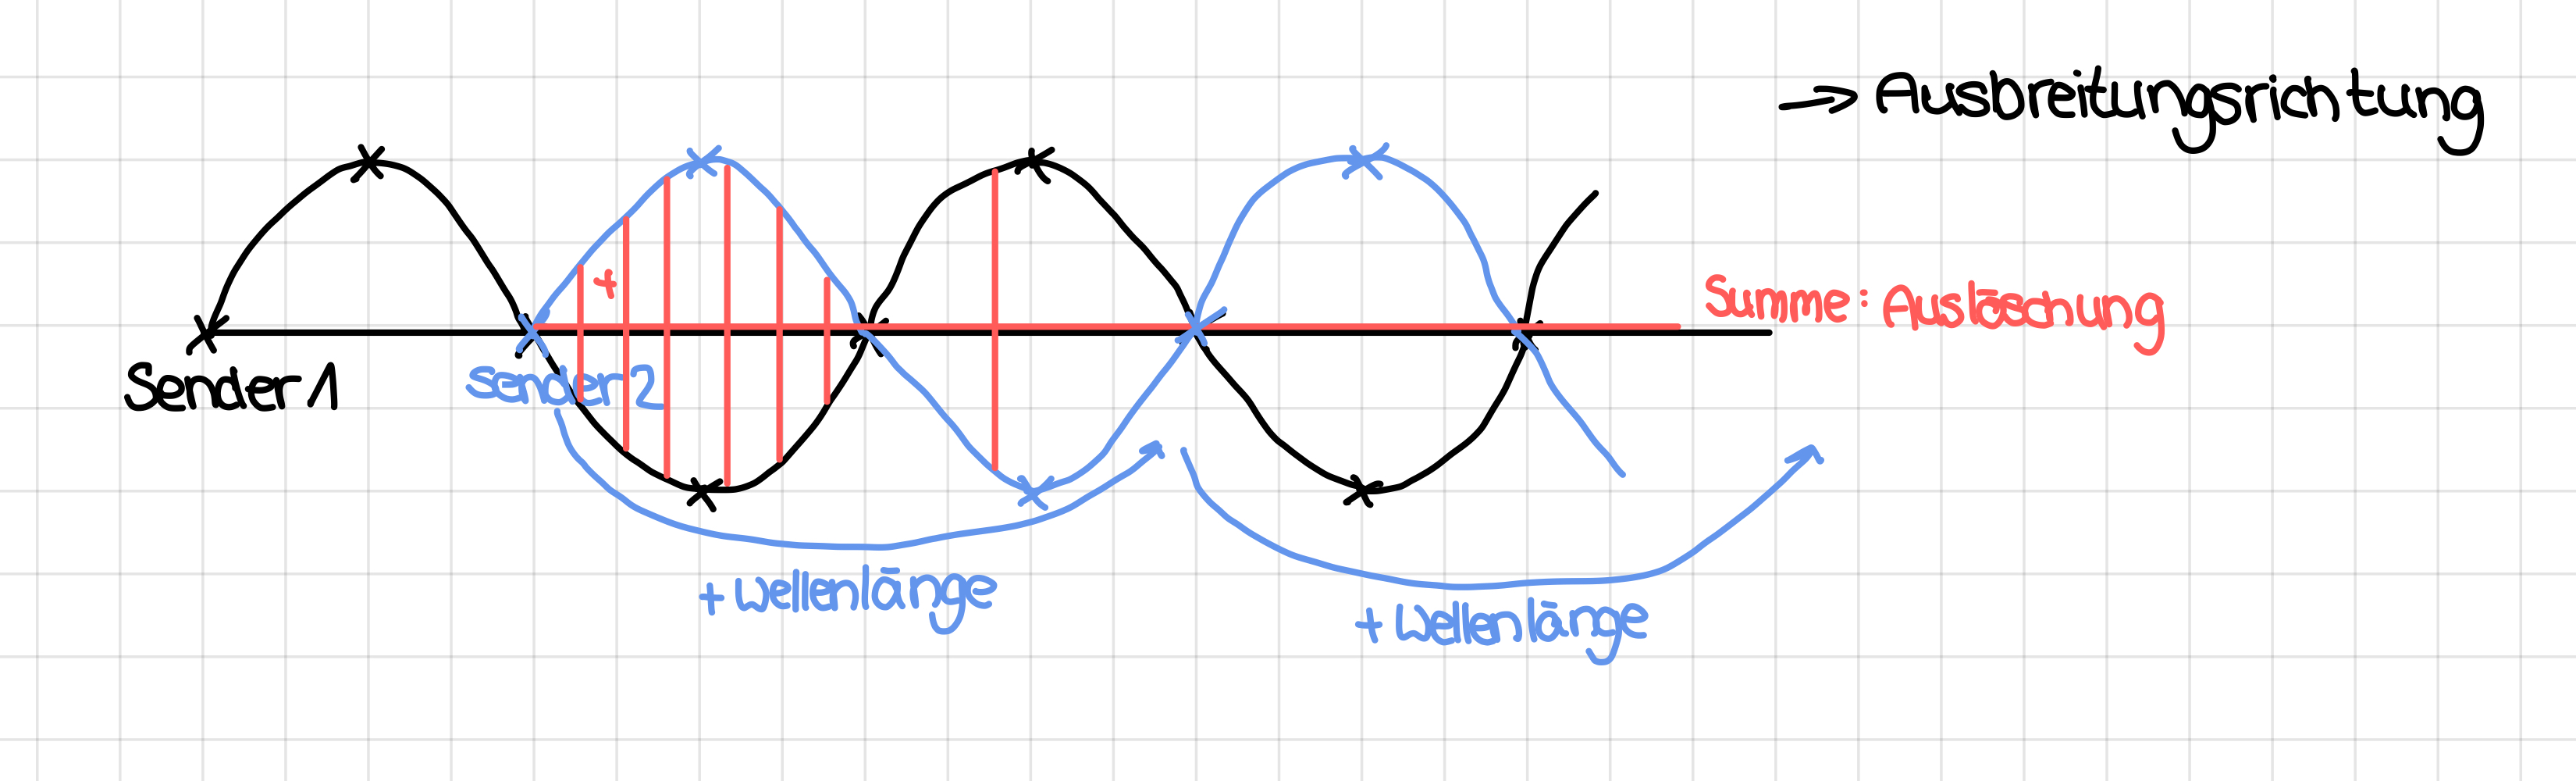
\includegraphics[width=\textwidth]{JPEG-Bild-443E-8313-20-0.JPEG}
	Eine Auslöschung (\dq Destruktive Interferenz\dq) erhalten wir, wenn wir die beiden Sender um eine halbe Wellenlänge (+ Vielfaches einer Wellenlänge) von uns entfernt stehen:
	\begin{align*}
		\bigtriangleup =n \cdot \lambda + \frac{\lambda}{2} &= \lambda \cdot (n+\frac{1}{2})
	\end{align*} \\
	Gangunterschied $\bigtriangleup$: \dq Weglängendifferenz\dq \\
	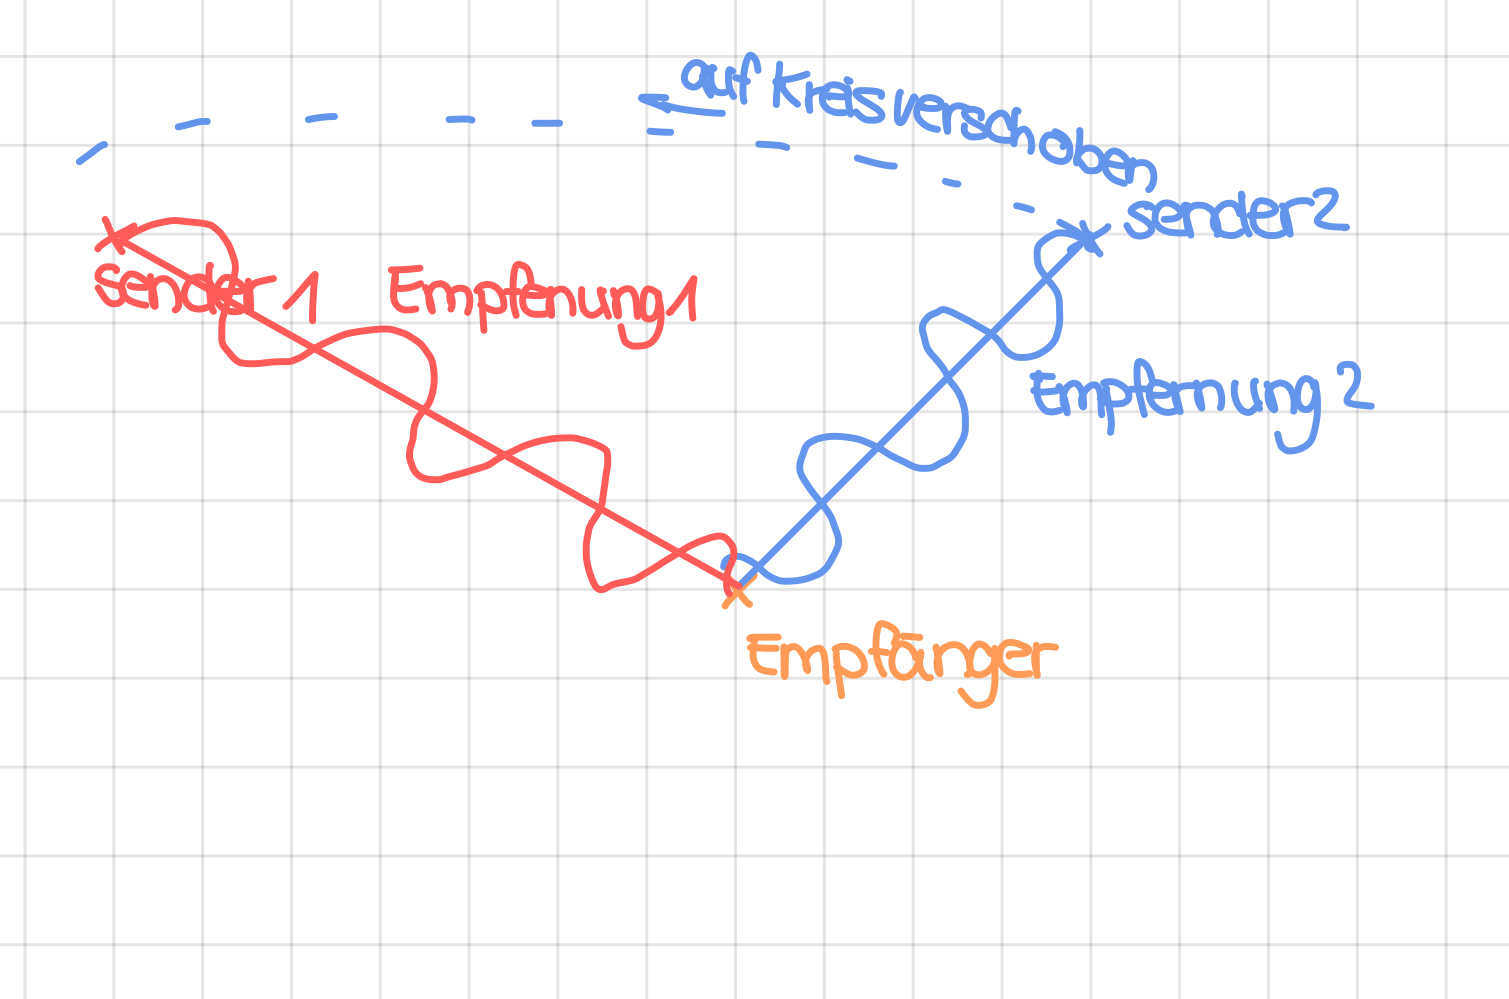
\includegraphics[width=\textwidth]{JPEG-Bild-4CCB-9E90-7A-0.JPEG}
	
\end{document}